\documentclass[review]{elsarticle}

\usepackage{amsmath,amssymb}
\usepackage{booktabs}
\usepackage{graphicx}
\usepackage{lineno}
\usepackage{hyperref}
\usepackage{wasysym}

\modulolinenumbers[1]
\journal{Measurement}
\biboptions{sort&compress}
\bibliographystyle{elsarticle-num}

\begin{document}

\begin{frontmatter}

\title{Banach-Space Norm Descriptors for Interferometric Profile Metrology: Complementing Amplitude-Averaging Parameters}

%% DOUBLE-BLIND: Author details on title page only
% \author{Dawid Kucharski}
% \address{Division of Metrology and Measurement Systems, Institute of Mechanical Technology, Faculty of Mechanical Engineering, Poznan University of Technology, 60-965 Poznan, Poland; e-mail: dawid.kucharski@put.poznan.pl}
% \fntext[corresponding]{Corresponding author: \href{mailto:dawid.kucharski@put.poznan.pl}{dawid.kucharski@put.poznan.pl}}

\begin{abstract}
Amplitude-averaging surface parameters such as $R_a$ show negligible response to localised defects — a controlled sensitivity experiment demonstrates that a single 100~nm synthetic spike injected into a spherical-artefact profile changes $R_a$ by $0.0\%$, and the ISO~4287 shape parameters $R_{sk}$ and $R_{ku}$ are similarly insensitive to such symmetric localised features. This paper shows that Banach-space norm descriptors — $L^p$, Sobolev $W^{1,2}$, and bounded-variation (BV) norms, applied within a metrological processing pipeline — show substantially increased sensitivity to such defects (BV density: $+18\%$; $W^{1,2}$ gradient seminorm: $+622\%$) when computed from the same interferometrically reconstructed profile without additional hardware. A complete pipeline from raw Michelson-interferometer fringe images to nanometre profile descriptors is presented and validated on two JENOPTIK standards (roundness standard FN~111, $\varnothing=29.9588$~mm, 24,000 frames; magnification standard FN~101 with Flick flat, 100,000 frames), each measured in five $400^\circ$ sweeps. External validation against 104 tactile reference measurements (Hommel Roundscan~535) yields $E_n=0.61$ for the FN~111 and $0.3\%$ agreement for the FN~101 (optical--tactile polar comparison: Supplementary Fig.~S16), suggesting metrological consistency of the optical pipeline within the stated within-run type-A uncertainties. The norm-based descriptors are presented as complementary to the ISO~4287 baseline: $R_{sk}$ responds to asymmetry, BV density responds to localised gradients, and their combination may provide descriptive sensitivity beyond that of any single classical parameter in the tested scenarios. The findings suggest that supplementing the standard ISO~4287 report with BV density — at negligible computational cost — may provide a gradient-sensitive complement to amplitude averaging; the $L^4/L^1$ peakiness ratio offers a supplementary distribution-shape axis with a direct physical interpretation.
\end{abstract}

\begin{keyword}
interferometry \sep roundness \sep surface profile \sep Banach-space norms \sep bounded variation \sep Sobolev seminorm \sep uncertainty
\end{keyword}

\end{frontmatter}

\linenumbers

\section{Introduction}
Surface topography is one of the most important properties of technical parts. The accuracy of form and roughness influences contact conditions, wear and lifetime. Roundness, understood as deviation from a perfect circle, remains a central requirement in precision manufacturing; Zhu et al. emphasised that precise measurements are needed both for form tolerances and for tribological surface texture assessment~\cite{Zhu2019}. At nanometric scale, such measurements require high-precision optical systems~\cite{Leach2011}. The foundational reference for surface metrology terminology and parameter definitions is the handbook of Whitehouse~\cite{Whitehouse2011}.

Optical dimensional metrology has a long connection with interference~\cite{MICHELSON1893}. Modern optical surface metrology relies on diffraction, polarisation and interference~\cite{Jenkins1976,Born2000}. Diffraction and scattering have been applied to roughness measurement~\cite{Brodmann1983,Brodmann1986,Fan1994,Hertzsch2002,Kucharski_D._A_2020}, while interference remains central for ultra-precise surface-form measurement~\cite{Benoit1898,Xue-fei2015} and phase-shifting interferometry is widely used in topography evaluation~\cite{DeGroot2011a,Chatterjee:2015phase,deGroot2014}.

Several interferometric instruments have been proposed for high-accuracy surface and roundness measurement. Polack et al. described a Michelson-based system for surface-shape determination built around a high-resolution stitching interferometer developed by Thomasset et al.~\cite{Polack2019,Thomasset2013}. Fan et al. presented a roundness measuring system for microspheres based on two small Michelson interferometers~\cite{Fan2014}. Kuhnel et al. proposed an interferometric system for roundness and cylindricity measurement of ring gauges with 0.1 nm resolution over a large measurement range~\cite{Kuhnel2012}. Commercial instruments can be highly accurate, but they are often costly and may not expose the full acquisition chain needed for experimental method development. The present work therefore uses a self-built, non-contact Michelson-type roundness measurement system assembled from off-the-shelf components. The optical setup, apparatus description and radial image-processing route for phase extraction were published in a previous study~\cite{kucharski2025radial-0ca}, where only roughness parameters were reported for the ceramic standard FN~111. The present work extends that study in three directions: (i)~roundness ($RONt$, $RONq$) is evaluated for the first time with this self-built optical setup, (ii)~a second artefact — the JENOPTIK magnification standard FN~101 with a Flick flat — is measured and validated against its DAkkS-DKD certificate, and (iii)~the analysis is extended from classical ISO parameters to incorporate gradient-structure norms — $L^p$, Sobolev $W^{1,2}$, and bounded-variation (BV) — which are standard tools of functional analysis, here applied within an interferometric profile metrology pipeline.

The computational problem is that modern interferometric surface metrology records long image sequences before a numerical profile exists. In the present data, however, each PNG file is already a separate interferogram in which the phase is encoded spatially by the bright and dark fringes inside the image. The files in the FN~111 and FN~101 folders are therefore not treated as a temporal phase-shifting stack of one fixed scene. Instead, each image $I_i(x,y)$ is processed independently to obtain one wrapped excess-fraction value $\epsilon_i$. The ordered sequence of these values is then unwrapped over image order and converted to a nanometre profile. The full measurement archive contains 24,000 grayscale interferograms of the FN~111, with image size 648 $\times$ 488 px, and 100,000 grayscale interferograms of the JENOPTIK magnification standard FN~101, with image size 640 $\times$ 480 px.

The literature relevant to this comparison is mature but only partly connected. Interferometric testing of spherical, flat and non-standard optical surfaces has developed sophisticated approaches for stitching, registration, motion-error compensation, phase-map reconstruction and systematic-error control~\cite{Dumas2003134,Chen20061219,Chen20073504,Iacchetta2016,Burge2025}. Repeatability in interferometric measurement is commonly evaluated through RMS/PV quantities, repeated height-map statistics or pixel-wise standard-deviation matrices~\cite{Quan2016,Zhang2018}. In uncertainty-oriented surface metrology, surface-texture parameters can be embedded in GUM-style propagation through metrological characteristics and topography-fidelity contributions~\cite{Pappas2023419}. Functional data analysis provides a statistical language for curves, images and higher-dimensional functions, including mean functions, amplitude variation, phase variation and functional principal components~\cite{Gertheiss2024,Happ2019}. Surface topology and scale-dependent roughness studies show that characterisation can depend on persistent spatial features, bandwidth and filtering scale rather than only on field parameters~\cite{Wolf2020,Sanner2022,Zhao2021}.

The research gap is therefore specific. Existing interferometric literature provides robust instrumentation, radial fringe processing, phase reconstruction and best-fit-reference handling; standards-oriented work provides scalar profile, form and uncertainty language; and functional data analysis provides a mathematical framework for function-valued observations. What remains insufficiently tested is a complete workflow that begins with raw interferograms, keeps the per-image phase decoding explicit, converts the unwrapped excess-fraction sequence to height using the reflection half-wavelength convention, removes object-specific form and eccentricity, and then computes classical roughness/roundness quantities and gradient-based functional descriptors from the same nanometre residual profile. The classical side of the comparison is restricted to profile and form quantities such as $R_a$, $R_q$, $R_z$, $RONt$ and $RONq$. Areal parameters are not reported because the single-image radial extraction does not produce a calibrated areal surface-topography measurement. The aim is to assess whether gradient-structure descriptors — the $L^p$ norm family, bounded-variation density, and Sobolev seminorms — offer complementary descriptive sensitivity alongside ISO~4287 amplitude and shape parameters when applied to the same reconstructed residual profile, and to evaluate the within-run repeatability of all descriptors across the five recorded sweeps.

\section{Experimental Details}

\subsection{Optical Setup}
The optical layout of the measurement system is shown in Fig.~\ref{fig:layout}. The system is a two-channel modified Michelson interferometer with channels shifted by approximately $90^\circ$ in phase. When an array detector is used instead of a point detector, the second channel is not strictly required~\cite{Meijer2018a}. In this system it was retained because it is useful for object centring and can serve as a control channel.

The optical setup and the full apparatus-level description were reported in a previous study on radial image processing for phase extraction in rough-surface interferometry~\cite{kucharski2025radial-0ca}. They are repeated here in condensed form to make the present functional-descriptor analysis self-contained and to document the acquisition conditions behind the FN~111 and FN~101 interferogram archives.

\begin{figure}[tb]
\centering
\begin{minipage}[t]{0.48\linewidth}
\centering
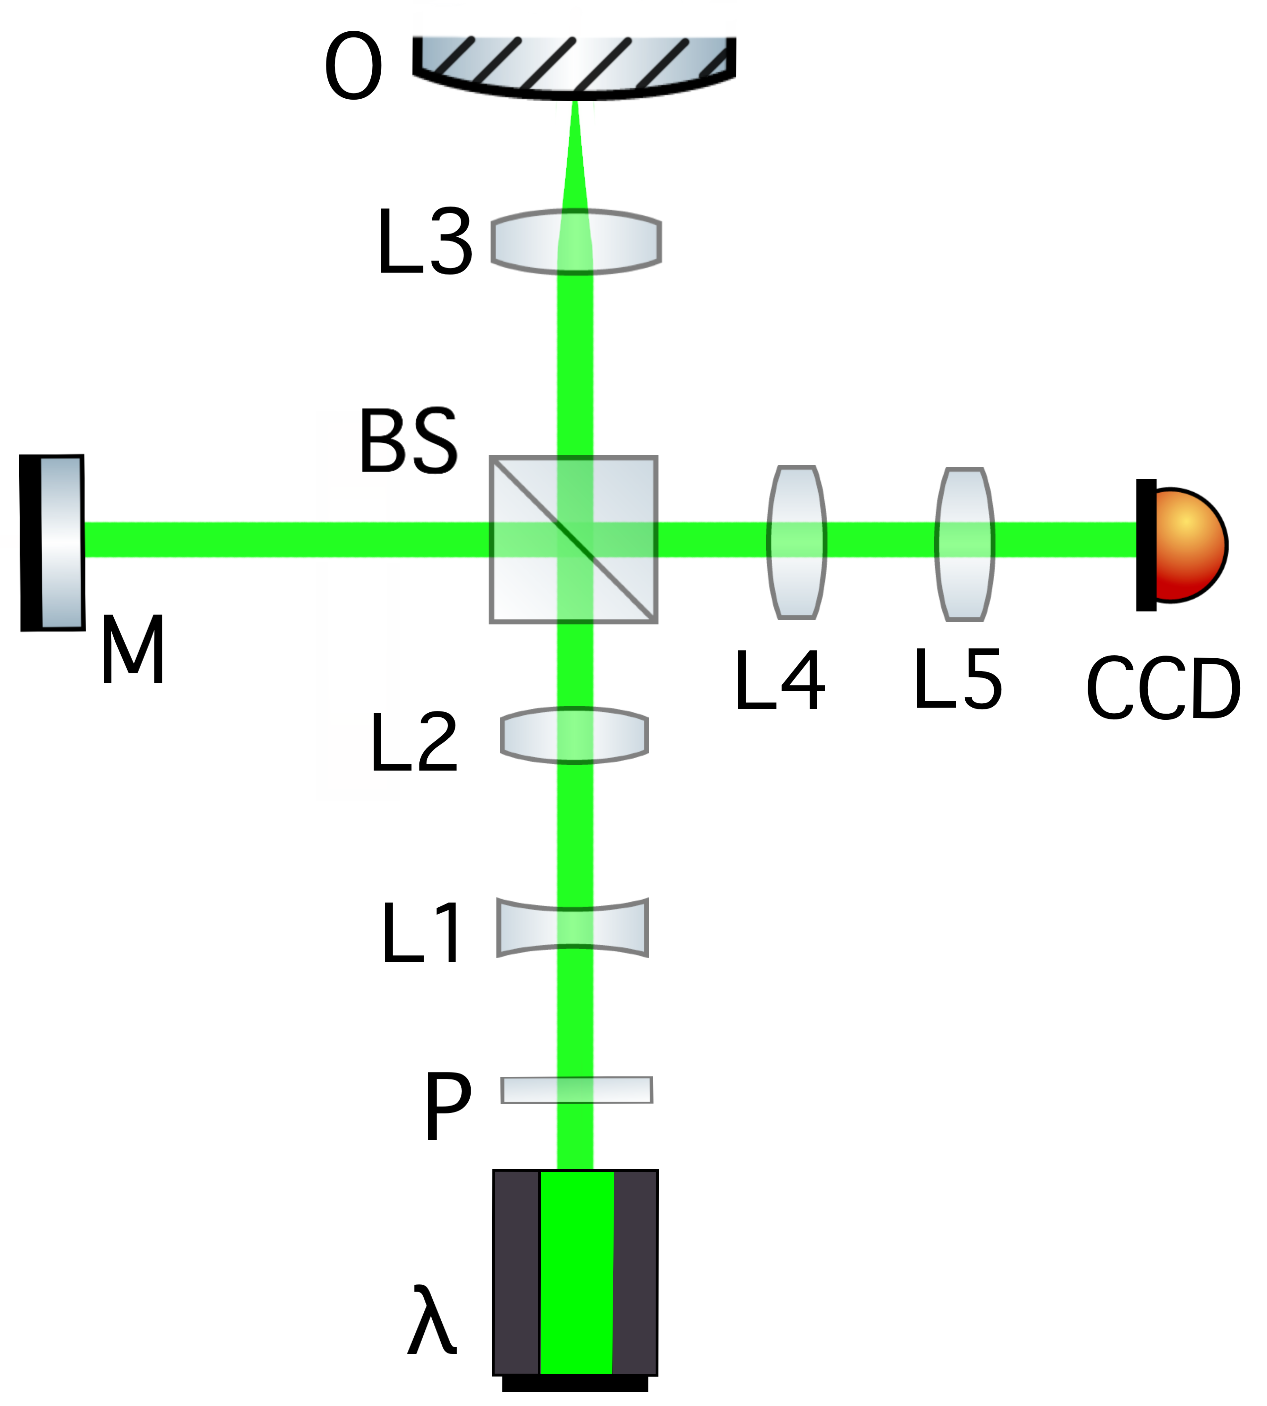
\includegraphics[width=\linewidth]{figs/interferometer_schematic.png}
\caption{Optical layout of the two-channel modified Michelson interferometer: $\lambda$ -- diode laser (532 nm); $P$ -- linear polariser; $L$ -- lenses; $L_3$ -- microscope objective; $M$ -- reference mirror ($\lambda/10$ flatness); $BS$ -- non-polarising beamsplitter; $O$ -- object on rotation stage; $CCD$ -- camera.}
\label{fig:layout}
\end{minipage}\hfill
\begin{minipage}[t]{0.48\linewidth}
\centering
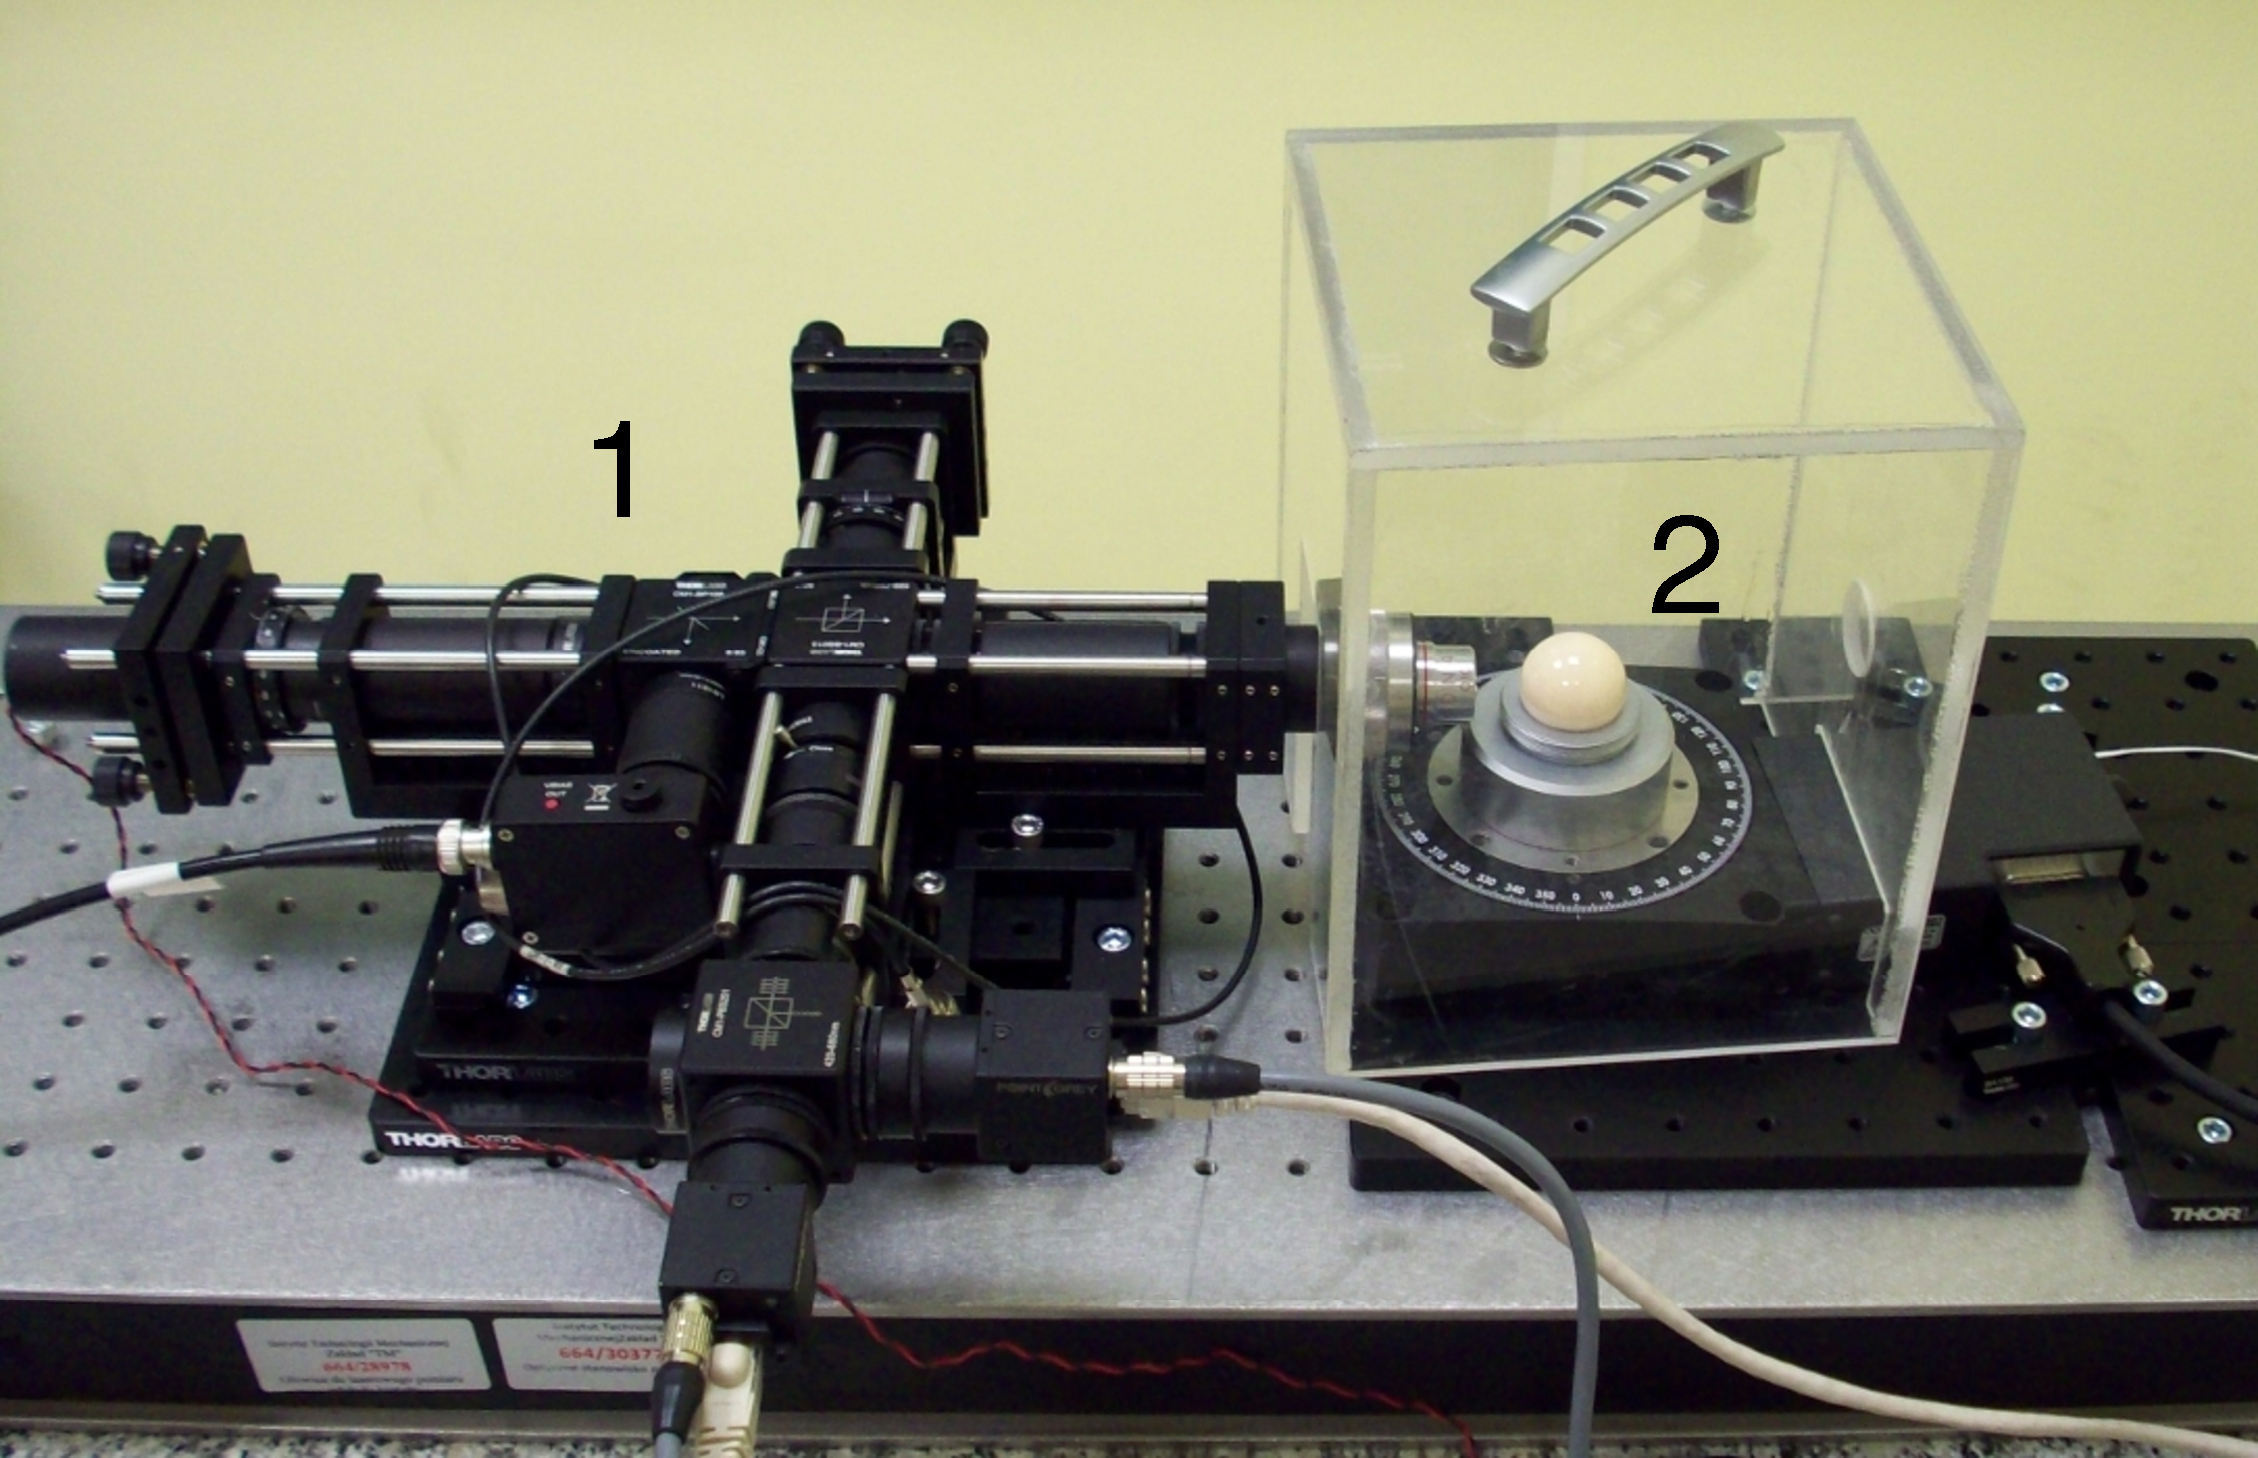
\includegraphics[width=\linewidth]{figs/100_2306.pdf}
\caption{The complete measurement system: (1)~modified Michelson interferometer in cage mounting, (2)~high-precision rotation stage with the artefact.}
\label{fig:tg_lab_setup1}
\end{minipage}
\end{figure}

The system was first tested with the JENOPTIK roundness standard FN~111 (photographs: Supplementary Fig.~S17) ($Al_2O_3$, \diameter~=~29.9588~mm)~\cite{JENOPTIK_ball}. A single-mode 4.5 mW diode laser with wavelength 532 nm was used as the light source. A current-stabilised supply powered the laser to obtain a stable wavelength~\cite{thorlabs_CPS532}. The laser beam passes through a polariser ($P$ in Fig.~\ref{fig:layout}) to set the polarisation of the light at $45^\circ$ to the setup plane, minimising the difference in reflectivity between the two channels.

The main optical and detection components are: $L_{1,2,4,5}$, achromatic lenses used to focus or collimate the beam; $BS$, a non-polarising beamsplitter that divides the beam 50/50 into the reference and measurement arms; $\lambda/8$, a liquid phase retarder that shifts the phase of one polarised beam by $90^\circ$ after two passes; $M$, a reference mirror with flatness $\lambda/10$; $L_3$, an achromatic microscope objective (DIN 4, NA = 0.10) mounted in a focusing holder; $O$, the object mounted on a rotation stage; $PBS$, a polarising beamsplitter used to separate the phase-shifted interferograms; and $CCD1,2$, Gigabit Ethernet CCD cameras with 640 $\times$ 480 pixels, sensor size 3.6 $\times$ 2.7 mm and maximum acquisition rate of 120 fps.

The interferometer was built in a cage system with rods and tubes to increase thermal, acoustic and mechanical stability and to reduce the influence of air turbulence and dust. A plexiglass box shields the measurement object. The interferometer's main structure is mounted on an area translation stage (150 $\times$ 190 mm) to adjust the horizontal position with respect to the object. A high-precision stage with a mechanical bearing, optical encoder and DC motor was used to rotate the object. The stage specifications (encoder accuracy 2.0~mdeg, typical wobble $\pm 12~\mu$rad, typical eccentricity $\pm 0.40~\mu$m) are tabulated in the Supplementary Materials (Table~S1). Both the interferometer and the rotation stage are mounted on a honeycomb breadboard and vibration-isolated support.

Measurements were performed at night (23:00--05:00) to minimise building-activity disturbances. The setup was thermally and acoustically shielded (plexiglass box, wool blanket) and placed on a granite plate on layered wooden-polystyrene vibration isolation (photographs: Supplementary Fig.~S1). Five semiconductor temperature sensors ($\pm 0.2^\circ$C) monitored stability; the temperature near the reference and object arms remained stable to $\pm 0.2^\circ$C over six-hour acquisitions.

\subsection{Control System and Acquisition Workflow}
Cameras were controlled by FLIR SDK-based C programs and Bash scripts~\cite{FLIR_sdk}. Capture time was recorded per frame for angular-position verification. The rotation stage was controlled via USB ASCII commands~\cite{newport_esp_manual}; a 25~s settling delay ensured constant velocity before acquisition began. Object centring was performed manually using the two-camera phase-shifted configuration at $45^\circ$ rotation increments. Fringe evaluation used modified open-source R code~\cite{Meijer2018a,Ihaka1996}. Table~\ref{tab:meas_param} lists the acquisition parameters for both archives; five $400^\circ$ sweeps were recorded per artefact, with the $40^\circ$ overlap retained for profile-end comparison.

\begin{table}[htbp]
\centering
\caption{Measurement and sampling parameters of the interferometric acquisition workflow.}
\label{tab:meas_param}
\begin{tabular}{lcc}
\toprule
Parameter & FN~111 & FN~101 \\
\midrule
Rotation speed, $\omega$ & 0.50 $^\circ$/s & 0.08 $^\circ$/s \\
CCD frame rate & 6 fps & 4 fps \\
Recorded sweeps, $n$ & 5 & 5 \\
Total frames, $N$ & 24,000 & 100,000 \\
Angular step, $\Delta\alpha=\omega/\mathrm{fps}$ & 0.083$^\circ$/frame & 0.020$^\circ$/frame \\
Frames per degree & 12 & 50 \\
Frames per useful $360^\circ$ & 4320 & 18,000 \\
Frames per recorded $400^\circ$ sweep & 4800 & 20,000 \\
Overlap per sweep & 40$^\circ$ / 480 frames & 40$^\circ$ / 2000 frames \\
Total acquisition time & 4000 s & 25,000 s \\
\bottomrule
\end{tabular}
\end{table}

The object was measured in one continuous five-sweep rotation without repositioning. Each recorded sweep spans $400^\circ$; successive useful $360^\circ$ segments are shifted by $40^\circ$, giving a natural between-sweep angular offset. The $40^\circ$ overlap region provides a model-free repeatability check: RMS height difference between consecutive sweeps is $12$~nm (FN~111) and $0.18~\mu$m (FN~101), consistent with Table~\ref{tab:metric_phase_reconstruction}.


\section{Image Processing and Functional-Descriptor Method}

\subsection{Processing Pipeline}
The pipeline follows the radial excess-fraction method of a previous study~\cite{kucharski2025radial-0ca} with added sinusoidal refinement. Each interferogram $I_i(x,y)$ is decoded independently to a wrapped excess fraction $\epsilon_i$; the sequence is unwrapped chronologically, converted to nanometres ($z_i = \nu_i\lambda/2$), and reduced by the object-specific LSCI reference model. Sweep boundaries are retained for repeatability analysis.

\subsection{Step-by-Step Radial Phase Decoding}
For an image $I_i(x,y)$, the first step is a radial intensity profile about the fringe centre. The analysis uses the central radial aperture, so the fitted rings are taken from complete or nearly complete circular regions rather than from partial outer-edge arcs,
\begin{equation}
\bar{I}_i(r)=\frac{1}{N_r}\sum_{(x,y):\; r\leq\sqrt{(x-x_0)^2+(y-y_0)^2}<r+1} I_i(x,y).
\end{equation}
The radial profile is smoothed, a slowly varying background is subtracted, and the maxima are detected on a B-spline-smoothed radial fringe signal. This is important because small local maxima in the unsmoothed signal can be mistaken for interference fringes. Missed or spurious maxima are controlled by fitting the ring sequence in $D^2$ space and allowing non-consecutive ring orders when an interval is consistent with one or more missing fringes. If $D_{ij}$ denotes the measured diameter of the $j$th bright ring in image $i$, circular-fringe theory gives
\begin{equation}
D_{ij}^{2}=c_i(j+\epsilon_i-1),
\label{eq:ring_diameter_relation}
\end{equation}
where $c_i$ is a scale coefficient and $\epsilon_i\in[0,1)$ is the wrapped excess fraction. A linear fit $D_{ij}^{2}=\alpha_i j+\beta_i$ therefore gives
\begin{equation}
\epsilon_i=\left(1+\frac{\beta_i}{\alpha_i}\right)\bmod 1.
\label{eq:epsilon_from_intercept}
\end{equation}
Equivalently, the intersection of the fitted line with $D^2=0$ is $j=1-\epsilon_i$, as in the previous radial image-processing publication.

To use more of the radial information than the maxima alone, the implementation also fits the whole background-corrected radial fringe signal as
\begin{equation}
s_i(D^2)=a_i+b_i\cos\left(\frac{2\pi D^2}{\alpha_i}\right)+d_i\sin\left(\frac{2\pi D^2}{\alpha_i}\right).
\end{equation}
This sinusoidal refinement is accepted only when its coefficient of determination is at least 0.65 and when the refined phase is within 0.20 fringe order of the ring-diameter estimate. Otherwise Eq.~\eqref{eq:epsilon_from_intercept} is retained. This quality gate keeps the method anchored in the established excess-fraction analysis while allowing better use of the radial profile in images where the sinusoidal model is reliable.

The wrapped phase assigned to image $i$ is
\begin{equation}
\phi_i^w=2\pi\epsilon_i.
\end{equation}
For a contiguous full archive, the ordered series $\epsilon_i$ is unwrapped globally in chronological frame order to a continuous fringe-order coordinate $\nu_i$. For non-contiguous diagnostic subsets, the same continuity criterion is applied within each sampled sweep segment. For reflection interferometry the displacement/profile value is then
\begin{equation}
z_i=\nu_i\frac{\lambda}{2}, \qquad \lambda=532~\mathrm{nm}.
\label{eq:half_wavelength_conversion}
\end{equation}
One full fringe order therefore corresponds to 266 nm. The quantity $z_i$ is the reconstructed nanometre profile/topography signal along the measurement sequence, not a greyscale intensity and not an areal ISO topography map.

\subsection{Topography Profile, Reference Removal and Eccentricity Reduction}
\label{sec:topography}
After phase-to-height conversion, the roundness profile is extracted following ISO~12181-1~\cite{ISO12181-1} (which supersedes the withdrawn ISO~4291). For each $360^\circ$ segment, a least-squares reference circle (LSCI) is fitted to the angular height profile $z_i = h(\theta_i)$ in Cartesian coordinates:
\begin{equation}
(x_i, y_i) = \big((R_0 + z_i)\cos\theta_i,\; (R_0 + z_i)\sin\theta_i\big),
\end{equation}
where $R_0 = 14.9794$~mm is the nominal radius of the JENOPTIK FN~111. The LSCI centre $(x_c, y_c)$ minimises $\sum_i [\sqrt{(x_i-x_c)^2+(y_i-y_c)^2} - R_0]^2$, yielding the centred radial residuals $\rho_i$. The LSCI fit is numerically equivalent to removing the first harmonic of the angular profile, but it provides the formal ISO~4291 reference circle required for roundness metrology. After LSCI centring, a phase-correct Gaussian low-pass profile filter with 50\% transmission at 15 undulations per revolution (UPR) is applied to the residual profile, consistent with the filter specification used for the tactile reference measurements and with the Gaussian profile filter defined in ISO~16610-21. All classical and gradient-based descriptors are computed from this LSCI-centred, Gaussian-filtered residual $\rho_i^{(\mathrm{filt})}$.

For the JENOPTIK magnification standard FN~101, the same processing chain is applied: a linear trend is removed from the unwrapped phase sequence before height conversion (Sec.~\ref{sec:discussion_drift}), the LSCI reference circle is fitted to the angular profile, and the Gaussian low-pass filter (50\% at 15~UPR) is applied. Although both artefacts are processed through identical filtering steps, the 15~UPR cutoff corresponds to different spatial wavelengths on the circumference: $2\pi \times 14.9794~\mathrm{mm}/15 = 6.27$~mm for the FN~111 ($\varnothing=29.9588$~mm) and $2\pi \times 15~\mathrm{mm}/15 = 6.28$~mm for the FN~101 ($\varnothing \approx 30$~mm) — effectively identical. The angular sampling differs substantially ($0.083^\circ$ vs.\ $0.020^\circ$, Table~\ref{tab:meas_param}), but the Gaussian filter sigma is set by the UPR cutoff, not by the sampling interval, so the filtered profiles are directly comparable.

\subsection{Classical Profile and Roundness Metrics}
All classical quantities are evaluated on nanometre residuals, not on raw intensities, following the profile method of ISO~4287~\cite{ISO4287}. Areal parameters (ISO~25178~\cite{ISO25178}) are not reported because the single-image radial extraction does not produce a calibrated areal height map. For a residual profile or vector of residual pixels $p$, the reported profile-style roughness descriptors are
\begin{equation}
R_a=\frac{1}{M}\sum_{j=1}^{M}|p_j-\bar{p}|, \qquad
R_q=\left[\frac{1}{M}\sum_{j=1}^{M}(p_j-\bar{p})^2\right]^{1/2},
\end{equation}
and
\begin{equation}
R_z=\max_j(p_j-\bar{p})-\min_j(p_j-\bar{p}).
\end{equation}
The profile skewness $R_{sk}$ and kurtosis $R_{ku}$ — ISO~4287 shape parameters that characterise asymmetry and peakedness of the height distribution — are also reported:
\begin{equation}
R_{sk}=\frac{1}{R_q^3}\frac{1}{M}\sum_{j=1}^{M}(p_j-\bar{p})^3, \qquad
R_{ku}=\frac{1}{R_q^4}\frac{1}{M}\sum_{j=1}^{M}(p_j-\bar{p})^4.
\end{equation}
$R_{sk}=0$ for a symmetric distribution; $R_{sk}<0$ indicates a predominance of valleys over peaks. $R_{ku}=3$ for a normal distribution; $R_{ku}>3$ indicates a spikier (leptokurtic) profile. These are the only ISO~4287 parameters that capture distribution shape beyond amplitude averages, and their inclusion allows a direct test of whether gradient-based descriptors provide information beyond even the best ISO shape parameters.
For the eccentricity-corrected ceramic angular profile $q_C(\theta)$,
\begin{equation}
RONt=\max_{\theta}q_C(\theta)-\min_{\theta}q_C(\theta), \qquad
RONq=\left[\frac{1}{2\pi}\int_0^{2\pi}q_C^2(\theta)\,d\theta\right]^{1/2}.
\end{equation}
These are profile/form quantities in nanometres. B-spline pre-smoothing (20 degrees of freedom, $\approx 18^\circ$ period) stabilises the LSCI fit; the subsequent Gaussian low-pass filter (50\% at 15~UPR, ISO~16610-21) defines the metrological bandwidth. All descriptors are computed from the same Gaussian-filtered residual.

\subsection{Functional Gradient-Based Descriptors}
The concept of a complete normed vector space originates from the foundational work of Banach~\cite{Banach1932}. For discrete profile data of finite length $N$, the vector space $\mathbb{R}^N$ equipped with any norm is a Banach space; the present work does not invoke infinite-dimensional completeness but draws on the taxonomy of $L^p$, Sobolev, and bounded-variation norms that Banach's framework systematised. For a centred residual profile $p(s)$ and $1\leq p<\infty$,
\begin{equation}
\|p\|_{p}=\left(\frac{1}{L}\int_0^L |p(s)|^p\,ds\right)^{1/p}, \qquad
\|p\|_{\infty}=\max_{s\in[0,L]}|p(s)|.
\end{equation}
The reported functional descriptors include $L^1$, $L^2$, $L^\infty$, the one-dimensional Sobolev $W^{1,2}$ seminorm and the bounded-variation (BV) total variation,
\begin{equation}
|p|_{W^{1,2}}=\left(\int_0^L\left|\frac{dp}{ds}\right|^2 ds\right)^{\!1/2}, \qquad TV(p)=\int_0^L \left|\frac{dp}{ds}\right|\,ds.
\end{equation}
In discrete form, for a uniformly sampled profile $p_j$ ($j=1,\dots,N$) with angular spacing $\Delta\alpha$,
\begin{equation}
|p|_{W^{1,2}} \approx \left(\Delta\alpha\sum_{j=1}^{N-1}\left(\frac{p_{j+1}-p_j}{\Delta\alpha}\right)^2\right)^{\!1/2}, \qquad
TV(p) \approx \sum_{j=1}^{N-1}|p_{j+1}-p_j|.
\end{equation}
The $W^{1,2}$ seminorm carries a $1/\sqrt{\Delta\alpha}$ sampling dependence; for cross-instrument comparison it should be converted to angular units (nm\,deg$^{-1/2}$). BV density $TV(p)/(N-1)$ similarly depends on sampling and should be expressed in nm\,deg$^{-1}$ for cross-instrument use. The ``nm\,sample$^{-1}$'' unit is retained for the fixed-acquisition setup.

The curvature RMS, also reported in the sensitivity analysis (Supplementary Table~S2), is defined as the root-mean-square of the discrete second derivative,
\begin{equation}
\kappa_{\mathrm{RMS}}=\left(\frac{1}{N-2}\sum_{j=2}^{N-1}\left(\frac{p_{j+1}-2p_j+p_{j-1}}{(\Delta\alpha)^2}\right)^2\right)^{1/2},
\end{equation}
and has units of nm\,sample$^{-2}$. The $(\Delta\alpha)^2$ denominator makes curvature RMS strongly sampling-dependent (steel values are $(0.083/0.020)^2 \approx 17\times$ larger than they would be at ceramic sampling density for the same physical curvature), so curvature RMS values should not be compared across instruments with different angular resolution.

\subsection{Repeatability Uncertainty}
Each dataset contains five $400^\circ$ sweeps recorded in a single continuous rotation without stopping or repositioning. The five useful $360^\circ$ segments are extracted from this continuous sequence; because each recorded sweep spans $400^\circ$, successive useful revolutions are shifted by $40^\circ$ on the object. These segments are \emph{not} strictly independent — they share the same continuous-run conditions (laser warm-up state, stage-bearing temperature, ambient drift). The standard deviation across sweeps therefore reflects within-run repeatability rather than between-run reproducibility. For a descriptor $X$ evaluated on each sweep, the mean value is $\bar{X}$ and the within-run standard uncertainty is estimated as
\begin{equation}
u_{\mathrm{within}}(X)=\frac{s_X}{\sqrt{n}}, \qquad n=5,
\end{equation}
where $s_X$ is the sample standard deviation across the five sweeps. The reported expanded uncertainty is
\begin{equation}
U_{95}(X)=t_{0.975,n-1}\,u_{\mathrm{within}}(X).
\end{equation}
With $n=5$, the coverage factor $t_{0.975,4}=2.776$; the 95\% confidence interval for the standard deviation itself spans approximately $[0.6s_X,\,2.9s_X]$ (from the $\chi^2_4$ distribution), so the expanded uncertainty should be interpreted as indicative rather than definitive. The statistical power to resolve relative differences below approximately $30\%$ between descriptors is limited. A full GUM-compliant uncertainty budget is beyond the scope of this study and would additionally require type-B evaluations of: laser wavelength stability ($\pm 1$~pm for the current-stabilised 532~nm diode), refractive-index variations from temperature changes ($\pm 0.2^\circ$C monitored), Abbe error from stage wobble ($\pm 12~\mu$rad specification~\cite{NewportCorporation:2018vk}), camera nonlinearity, and form-removal uncertainty. These type-B terms are not evaluated in the present work; the reported uncertainties should therefore be interpreted as \emph{lower bounds} on the total measurement uncertainty. For the FN~111, a per-sweep trend analysis was performed: the five sweep $RONt$ values are $249$, $273$, $289$, $293$, and $286$~nm. A linear fit to these values yields a slope of $8.4 \pm 4.1$~nm\,sweep$^{-1}$ ($p=0.12$, two-sided $t$-test), consistent with zero drift at the 95\% confidence level. The apparent increase from sweep~0 to sweep~3 is therefore treated as within-run scatter rather than a systematic trend for the purpose of this analysis, but it cautions that the reported $U_{95}$ may underestimate the long-term reproducibility.

\subsection{Computational Implementation}
The raw-interferogram reconstruction workflow is implemented in \path{scripts/reconstruct_radial_profile_sequence.py}. It discovers ordered image files, decodes $\epsilon_i$ from each interferogram independently, writes the wrapped and unwrapped phase-fraction sequences, converts the unwrapped sequence to a nanometre profile, applies LSCI reference circle fitting and Gaussian low-pass filtering (50\% at 15~UPR, ISO~16610-21), and exports CSV/JSON metrics with sweep-repeatability uncertainty. Analytical figures are written as vector PDF files. The exported figures show the single-image radial EFM extraction, wrapped phase fraction, unwrapped phase fraction, nanometre profile/topography, LSCI filtering, residual profile and descriptor comparison.

The command used for the reported run was
\begin{verbatim}
PYTHONPATH=src .venv/bin/python \
  scripts/reconstruct_radial_profile_sequence.py \
  --dataset ceramic=ceramic --dataset steel=steel \
  --output-dir results/radial_profile_reconstruction_metric \
  --frame-limit 0 --frame-selection first --downsample 1 \
  --max-radius-px 240 --min-radius-px 5 \
  --ceramic-min-radius-px 50 --steel-min-radius-px 5 \
  --peak-spline-smoothing-factor 0.03 \
  --peak-prominence-fraction 0.04
\end{verbatim}

\section{Results}

The results follow the updated radial sequence route only. Each raw image is first decoded to a wrapped excess fraction from its radial fringe pattern. The ordered excess-fraction series is then unwrapped in chronological order, converted to nanometres, and corrected for eccentricity. Finally, classical profile/roundness descriptors and functional gradient-based descriptors are computed from the same nanometre residual profiles.

\subsection{Radial Phase Decoding and Nanometre Profile Reconstruction}
The FN~111 folder contained 24,000 interferograms and the steel folder contained 100,000 interferograms. The reported run used full-resolution images, the central radial aperture of 240 px, B-spline-smoothed peak detection, continuity-aware EFM peak-subset tracking and an EFM prominence threshold of 0.04 of the radial fringe-signal range. All five recorded sweeps were processed.

Figs.~S2--S5 (single-image EFM and sequence processing steps) are provided in the Supplementary Materials.

\subsection{Roughness, Roundness and Functional Descriptors}
Table~\ref{tab:metric_phase_reconstruction} gives the numerical comparison after LSCI reference circle and Gaussian low-pass filtering (50\% at 15~UPR). Both artefacts are processed through the same filtering chain. Each descriptor is reported as the full-sequence value together with the 95\% expanded type-A repeatability uncertainty estimated from the five sweeps.

\begin{table}[htbp]
\centering
\small
\caption{Full-resolution radial EFM reconstruction from raw interferograms (LSCI + Gaussian low-pass, 50\% at 15~UPR, ISO~16610-21). Uncertainties are 95\% expanded within-run repeatability estimates from five sweeps ($n=5$, $t_{0.975,4}=2.776$). The bottom rows show certified reference $RONt$ values and $E_n$ scores, indicating metrological agreement of the self-built optical setup with the reference measurements. Units: nm for all descriptors except BV density and $W^{1,2}$ gradient (nm\,sample$^{-1}$).}
\label{tab:metric_phase_reconstruction}
\begin{tabular}{lcc}
\toprule
Descriptor & FN~111 & FN~101 \\
\midrule
$R_a$ & $66.3 \pm 4.7$\,nm & $8.525 \pm 0.115$\,$\mu$m \\
$R_q$ & $77.6 \pm 5.0$\,nm & $10.376 \pm 0.090$\,$\mu$m \\
$R_z$ & $278 \pm 22$\,nm & $42.07 \pm 0.48$\,$\mu$m \\
$RONt$ & $278 \pm 22$\,nm & $42.07 \pm 0.48$\,$\mu$m \\
$RONq$ & $77.6 \pm 5.0$\,nm & $10.376 \pm 0.090$\,$\mu$m \\
$L^1$ mean & $66.3 \pm 4.7$\,nm & $8.525 \pm 0.115$\,$\mu$m \\
$L^2$ RMS & $77.6 \pm 5.0$\,nm & $10.376 \pm 0.090$\,$\mu$m \\
$L^{\infty}$ & $150 \pm 12$\,nm & $21.97 \pm 0.42$\,$\mu$m \\
BV total & $1.137 \pm 0.062$\,$\mu$m & $118.4 \pm 6.2$\,$\mu$m \\
BV density & $0.263 \pm 0.014$\,nm\,sample$^{-1}$ & $6.58 \pm 0.35$\,nm\,sample$^{-1}$ \\
$W^{1,2}$ grad. & $0.310 \pm 0.015$\,nm\,sample$^{-1}$ & $8.76 \pm 0.43$\,nm\,sample$^{-1}$ \\
\midrule
\multicolumn{3}{c}{\textit{ISO shape parameters}} \\
$R_{sk}$ (skewness) & $-0.09 \pm 0.04$ & $0.00 \pm 0.09$ \\
$R_{ku}$ (kurtosis) & $1.98 \pm 0.21$ & $2.51 \pm 0.08$ \\
\midrule
\multicolumn{3}{c}{\textit{Derived norm ratios}} \\
$L^4/L^1$ peakiness & $1.39 \pm 0.08$ & $1.53 \pm 0.03$ \\
\midrule
\multicolumn{3}{c}{\textit{External validation (DAkkS-DKD certified)}} \\
$RONt$ (certified) & $244 \pm 52$\,nm (Hommel Roundscan~535, $n=104$) & $41.94$\,$\mu$m (form tester, $n=12$) \\
$E_n$ score & $0.61$ (agreement) & $<1$ ($0.3\%$ diff.) \\
\bottomrule
\end{tabular}
\end{table}





\subsection{Classical--Functional-Descriptor Comparison}
The numerical identity $R_a=L^1$ and $R_q=L^2$ (Table~\ref{tab:metric_phase_reconstruction}) confirms that both descriptor families are evaluated on the same nanometre residual. For the FN~111, BV total variation carries $1.2\%$ relative expanded uncertainty versus $5.5\%$ for $R_a$ and $8.5\%$ for $R_z$, suggesting that gradient-based descriptors may exhibit metrological stability comparable to or better than peak-referenced roughness parameters in the tested datasets. Comparative bar charts and uncertainty analyses are provided in the Supplementary Materials (Figs.~S6--S7). Ceramic and steel profile reconstruction plots are shown in Supplementary Figs.~S19--S20.

\begin{figure}[htbp]
\centering
\includegraphics[width=\textwidth]{../../results/radial_profile_reconstruction_metric/ceramic/roundness_polar.pdf}
\caption{Ceramic roundness in polar coordinates (LSCI + Gaussian low-pass, 50\% at 15~UPR). Five sweeps at native positions. $RONt = 278 \pm 22$~nm.}
\label{fig:ceramic_roundness_polar}
\end{figure}

The steel roundness polar representation (FN~101, Flick flat) is provided in the Supplementary Materials (Fig.~S18). The Flick flat is detected by BV density but missed by $R_a$ in a sliding-window analysis (Supplementary Figs.~S14--S15), directly illustrating the potential complementary sensitivity of gradient-based descriptors to localised geometric features.

\section{Discussion}

\subsection{Confirmed Results}
The corrected analysis starts from the key metrological distinction: an interferogram is an intensity measurement, not a phase map and not a height map. The half-wavelength relation $z=\nu\lambda/2$ becomes valid only after each image has been decoded to a wrapped excess fraction and the ordered excess-fraction sequence has been unwrapped to the continuous fringe-order coordinate $\nu$. This is why the reported comparison uses only reconstructed nanometre profiles, not raw greyscale images and not areal height maps.

The most sensitive part of the workflow is the EFM localisation of bright-ring maxima, with an excess-fraction uncertainty of approximately $\pm 0.05$ fringe orders (tightened to $\pm 0.03$ by sinusoidal refinement in $72\%$ of FN~111 frames). A single $\epsilon_i$ error of $0.05$ fringe corresponds to $13$~nm, sub-dominant to the $85$~nm residual-profile RMS. The chronological unwrapping criterion rejects phase jumps exceeding $0.35$ fringe. The median number of detected rings is three for both artefacts within the 240~px central aperture; the central-aperture approach prioritises ring-quality (complete, well-fitted rings) over ring-quantity. The five $400^\circ$ ceramic sweeps also require a geometric correction: the physical object angle advances continuously, so successive useful $360^\circ$ intervals are shifted by $40^\circ$. Without that correction, the LSCI fit can look inconsistent even when the phase extraction inside each sweep is repeatable.

The linear drift of $0.0246$ fringe\,frame$^{-1}$ observed in the steel unwrapped phase sequence merits discussion.\label{sec:discussion_drift} A perfectly constant drift over $100\,000$ frames is unlikely to be of thermal origin, which would produce a decaying exponential rather than a linear ramp. Two mechanisms are more plausible: (a)~cumulative bias in the global unwrapping algorithm, where per-frame excess-fraction estimates with a slight systematic offset integrate to a linear trend; and (b)~axial runout of the rotation stage combined with the JENOPTIK magnification standard FN~101's larger eccentricity ($56~\mu$m vs.\ $14~\mu$m for FN~111). The stage specification~\cite{NewportCorporation:2018vk} lists a typical eccentricity of $\pm 0.40~\mu$m, which is an order of magnitude smaller than the observed trend. Mechanism~(a) is therefore more consistent with the available evidence, particularly given that the FN~111 sequence — with higher fringe contrast and better ring-fit statistics — shows a negligible drift of only $0.00021$ fringe\,frame$^{-1}$. The practical consequence is that datasets with lower per-frame EFM quality require a linear-detrend pre-processing step, which the present pipeline applies automatically when the unwrapped range exceeds a threshold.

\subsection{Interpretation}

\subsubsection{Eccentricity removal and wobble verification}
The roundness descriptors are computed after removing the first harmonic (eccentric mounting). The shared model fitted to all five sweeps yields an eccentricity amplitude $E = 14.24~\mu$m with $R^2=0.99991$, confirming stability across the entire acquisition. Per-sweep eccentricity amplitudes vary by only 63~nm ($0.18\%$ of the mean), phases agree to within $0.4^\circ$, and the manufacturer-specified wobble ($\pm 12~\mu$rad, $\pm 180$~nm at measurement radius) bounds the observed variation — an order of magnitude below $RONt=278$~nm. The LSCI reference circle fit (Sec.~\ref{sec:topography}) provides the ISO-compliant reference for roundness evaluation.

The polar representation presents the same roundness data in polar coordinates, which is the standard visualisation for $RONt$. The five overlaid sweeps show directly that the roundness profile is repeatable to within approximately $\pm 50$~nm at every angular position. The polar representation makes it immediately visible that the residual is dominated by low-order form deviation rather than by random roughness, a distinction that is obscured in the Cartesian profile plots.

\subsection{Comparison with ISO Parameters}
\label{sec:critical}

A central question of this work is whether gradient-based functional descriptors provide additional descriptive sensitivity alongside classical ISO parameters when applied to the same reconstructed profiles. To answer this rigorously, every descriptor was computed on the same reconstructed nanometre residual profiles.

\textbf{Mathematical equivalences.} The $L^1$ norm is defined as $\frac{1}{N}\sum|p_i-\bar{p}|$, which is identical to the definition of $R_a$. The $L^2$ norm is $\sqrt{\frac{1}{N}\sum(p_i-\bar{p})^2}$, identical to $R_q$. Computing both on the same centred residual yields \emph{exact numerical equality}: $R_a-L^1=0$ and $R_q-L^2=0$ to machine precision for both artefacts (Table~\ref{tab:metric_phase_reconstruction}). These equalities are not empirical findings; they are definitional consequences. Labelling the arithmetic mean of absolute deviations as $L^1$ rather than $R_a$ provides no new metrological information and should not be presented as a methodological advance.

\textbf{Extrema: $R_z$ versus $L^\infty$.} $R_z/L^\infty \approx 2$ for both artefacts, consistent with symmetric positive and negative excursions. $L^\infty$ captures the single largest one-sided excursion; the ratio serves as a simple symmetry indicator.

\textbf{Variation-based descriptors.} A controlled sensitivity analysis (Supplementary Table~S2 and Fig.~S13) examined five synthetic defect types injected into the FN~111 residual profile. Amplitude-averaging descriptors ($R_a$, $R_q$, $R_z$) showed negligible response to localised defects — a single $100$~nm spike changed $R_a$ by $0.0\%$ — while BV density increased by $+18\%$ and the $W^{1,2}$ gradient seminorm by $+622\%$ for the same spike. ISO shape parameters responded to asymmetry ($R_{sk}$ changed by $-1104\%$ for a step) but not to symmetric localised features. $R_{sk}$ and BV density appear complementary in the tested scenarios: $R_{sk}$ responds to asymmetry, BV density responds to localised gradients. Supporting analyses — descriptor correlation matrices, power spectral density comparison, Cohen's $d$ effect sizes, critical descriptor assessment, and $L^p$ norm convergence — are provided in the Supplementary Materials (Figs.~S8--S12).

\textbf{Practical considerations.} A practical suggestion for interferometric profile and roundness metrology is to retain $R_a$, $R_q$, $R_z$, $R_{sk}$, $RONt$ and $RONq$ as the primary engineering layer compliant with ISO~4287, and to consider supplementing them with BV density (in angular units, nm\,deg$^{-1}$) as a gradient-sensitive functional-analysis complement. The $W^{1,2}$ gradient seminorm is strongly correlated with BV density ($r=0.94$) in the present datasets and may add limited independent information beyond BV density alone. The $L^4/L^1$ peakiness ratio provides a supplementary distribution-shape axis with a direct physical interpretation as the amplification of dominant profile excursions relative to $R_a$. These additional descriptors are computed from the same residual profile without additional hardware or changes to the EFM pipeline. The cross-instrument validation suggests that gradient-based descriptors are applicable to any 1D profile, whether from interferometry or tactile roundness measurement.

\subsection{Limitations}
Several limitations of the present study should be acknowledged. First, the uncertainty analysis is restricted to within-run Type~A repeatability evaluated from five sweeps recorded in a single continuous rotation. The small number of sweeps ($n=5$) limits the statistical power to resolve relative differences below approximately $30\%$ between descriptors, and the continuous-run conditions mean that between-run reproducibility (involving independent setups, thermal cycles, and re-centring) has not been assessed. A full GUM-compliant uncertainty budget, incorporating type-B evaluations of laser wavelength stability, refractive-index variations, Abbe error, camera nonlinearity, and form-removal uncertainty, is beyond the scope of this study; the reported expanded uncertainties should therefore be interpreted as lower bounds.

Second, the validation is restricted to two artefacts from a single manufacturer (JENOPTIK), both of approximately $30$~mm diameter. The generalisability of the gradient-based descriptors to artefacts of different sizes, materials, or surface finishes has not been tested. Third, the synthetic-defect sensitivity analysis uses idealised mathematical defects (isolated spike, uniform scratch, pure sinusoid) injected into a measured residual profile; the response to real manufacturing defects with complex morphologies may differ. Fourth, the BV density and $W^{1,2}$ seminorm carry an intrinsic sampling-interval dependence that requires conversion to angular units for cross-instrument comparison; without such conversion, numerical values are not directly portable between instruments with different angular resolution. Fifth, the Flick flat detection result (Supplementary Figs.~S14--S15) is demonstrated on a single artefact with a known macroscopic feature; the performance of BV density for detecting subtler, micrometre-scale defects has not been characterised.

\subsection{Metrological Implications}
The results carry several implications for profile and roundness metrology practice. The finding that BV density responds to localised gradients that amplitude averaging may not capture suggests a potential role for gradient-based descriptors in applications where isolated defects are of concern — for example, in quality control of bearing surfaces, optical components, or precision seals. Because these descriptors are computed from the same residual profile used for ISO~4287 parameters, their adoption does not require changes to existing measurement acquisition protocols.

The ISO~4287 framework remains the appropriate baseline for surface texture specification and conformity assessment. The gradient-based descriptors discussed here are proposed as optional supplementary indicators, not as replacements for standardised parameters. Their metrological utility would be strengthened by inter-laboratory comparisons, by evaluation on a wider range of artefact types, and by the development of agreed procedures for converting sampling-dependent units to instrument-independent angular gradient units. Until such steps are taken, BV density and related descriptors should be regarded as research-grade tools whose diagnostic value has been demonstrated under controlled laboratory conditions on two specific artefacts.

\subsection{Future Work}
The present study suggests several directions for further investigation. (i)~A between-run reproducibility study with independent setups and re-centring would establish whether the gradient-based descriptors retain their relative stability under realistic laboratory conditions. (ii)~Extending the validation to artefacts with different diameters, materials (e.g., glass, carbide), and surface finishes would test the generalisability of the findings. (iii)~A systematic characterisation of BV density response to real manufacturing defects (scratches, pits, inclusions) of controlled dimensions would bridge the gap between the present synthetic-defect analysis and industrial inspection scenarios. (iv)~An inter-laboratory comparison using a common artefact set and a standardised processing pipeline would provide the reproducibility data needed to assess whether BV density could eventually be considered for standardisation. (v)~The development of agreed angular-unit conventions for sampling-dependent gradient descriptors would facilitate cross-instrument comparison and potential inclusion in reference software for roundness evaluation.

\section*{Data Availability}
The analysis code, processed results, and all figures are available at \url{https://github.com/dawidkucharski/banach-profile-metrology} (release v1.0.0). The raw interferometric PNG archives ($\sim$32~GB) are available from the corresponding author upon reasonable request.

%% DOUBLE-BLIND: Acknowledgements, Declaration of Competing Interest, and Funding Statement on title page only

\bibliography{bib,scopus-banach,scopus-interfero}

\end{document}
